\documentclass[pdftex,12pt,a4paper]{report}

% Some useful packages.
\usepackage{amsmath}
\usepackage{siunitx}
\usepackage{graphicx}
\usepackage{verbatim}
\usepackage{mhchem}
\usepackage{textcomp}
\usepackage{setspace}

% Reduces margins substantially.
\usepackage{geometry}
\newgeometry{margin=3.0cm}

% Allows headers and footers.
\usepackage{fancyhdr}
\pagestyle{fancy}
% Get rid of annoying line under header.
\renewcommand{\headrulewidth}{0pt}

% Temporary fix for missing font problem.
% N.B. I know this is wrong, but there is a problem with missing fonts otherwise.
\renewcommand{\textdegree}{$^{\circ}$ } 

\lhead{}
\chead{}
\rhead{}

\newcommand{\ts}{\textsuperscript}
\newcommand{\HRule}{\rule{\linewidth}{0.5mm}}

% Harvard style references.
\usepackage[backend=biber,style=authoryear,sorting=nyt,dashed=false]{biblatex}
\renewcommand*{\nameyeardelim}{\addcomma\space}
\addbibresource{references/references.bib} % note the .bib is required

%\newcommand{\coo}{\ce{CO2}}

% 12,000 words max.

% overall structure:
% Abstract
% Intro
% Data Sources
% Development of the Hurricane Detection Algorithm
% Conclusion
% Appendices
% References

\title{Objective Tracking and Classification of Hurricanes in the 20\ts{th} Century Reanalysis Dataset}
\author{Mark Muetzelfeldt - UCL Department of Geography}

\date{29 August, 2014}

\begin{document}

\begin{titlepage}

\begin{center}

\textsc{\LARGE University College London}\\[1.5cm]

\textsc{\Large MSc Environmental Modelling Dissertation}\\[0.5cm]

% Title
\HRule \\[0.4cm]
{ \LARGE \bfseries Objective Tracking and Classification of Hurricanes in the 20\ts{th} Century Reanalysis Dataset \\[0.4cm] }

\HRule \\[1.5cm]

% Author and supervisor
\begin{minipage}{0.4\textwidth}
\begin{flushleft} \large
\emph{Author:}\\
Mark \textsc{Muetzelfeldt}
\end{flushleft}
\end{minipage}
\begin{minipage}{0.4\textwidth}
\begin{flushright} \large
\emph{Supervisors:} \\
Dr.~Chris \textsc{Brierley} \\
Qinling \textsc{Wu}
\end{flushright}
\end{minipage}
\\[0.5cm]
29\ts{th} August, 2014
\\[0.5cm]

This research dissertation is submitted for the MSc Environmental Modelling at University College London


\vfill
% Bottom of the page

\end{center}

\end{titlepage}


% Should be >= 400 words.
% Not included in word count.

\onehalfspacing
\section*{Abstract}

From an ...

\begin{center}
\textbf{Word count:} TODO
\end{center}

\section*{Acknowledgements}

I would like to thank Dr. Chris Brierley for his guidance and assistance in this dissertation.
Technical expertise from Qinling Wu proved useful in setting the direction for this project. 
Talking to Joshua Studholme helped to provide context for the field and ideas for analysis. % CLUMSY
Meeting Dr. Kevin Hodges (Reading University) was useful for [tracking help]. 
Finally, numerous discussions with Robert Muetzelfeldt were invaluable for keeping me on track and
for sounding out various ideas.

\newpage

\tableofcontents

% Everything from here to auto-critique is included in word count.
\chapter{Introduction}
% Introduction, presenting the research problem, rationale, context and outline objectives,
% aims/objectives (possibly as a formal hypothesis).

\section{Research Problem}

However \textcite{walshObjective1997} have found that \dots

\subsection{Rationale}

\subsection{Context}

% Finish with a run-down of the structure of the rest of the dissertation, including why it deviates
% from the traditional Intro/Methods/Results/Discussion/Conclusion structure.

\chapter{Data Sources}

\section{20\ts{th} Century Reanalysis Project}
The 20\ts{th} Century Reanalysis Project (20CRP) is a project whose aim is to produce a best estimate of
the state of the atmosphere by including information from a variety of different sources using data
assimilation \parencite{compoTwentieth2011}.

\section{IBTrACS Best Tracks Dataset}
The International Best Track Archive for Climate Stewardship (IBTrACS) 
\parencite{knappInternational2010} is a 

% TODO: chapter title?
\chapter{Development of the Hurricane Detection Algorithm}

% Overall description to go here, with flow chart.
% Mention: 
% * project URLs
% * choice of tracking then classification vs classifying individual CDPs
% * amount of processing required

\section{Data Processing}

\subsection{Wind Fields and Vorticity}

In the 20CRP data, the longitudinal and latitudinal wind fields, $u$ and $v$ respectively, were used
to calculate the vorticity and wind speeds. These are available at three different pressure levels:
\SI{995}{hPa}, \SI{850}{hPa} and \SI{250}{hPa}. The \SI{250}{hPa} fields were only used to determine
whether or not they were suitable for tracking of hurricanes, and it was found that they did not
produce suitable tracks, and were not further used (see Section \ref{sec:results_tracking}). The
formula for vorticity, $\omega$, is given by:

\begin{equation}
    \omega = \frac{\partial v}{\partial x} - \frac{\partial u}{\partial y}
    \label{eqn:vorticity}
\end{equation}

The surface of the earth, $R_e$, is taken as its mean radius of \SI{6371}{km}, and $\phi$, $\lambda$ 
denote the latitude and longitude coordinates. $u_{i, j}$ denotes the longitudinal wind speed at
grid cell $i, j$. Then $\omega$ can approximated on the surface of the Earth using a 2\ts{nd} order
approximation: %CLUMSY

% Calculation in code is a little different because it uses degrees instead of radians:
% More like vorticity = du / (2 * dlon * cos(lat * pi / 180) * Earth_circ / 360) - dv / ((2 * dlat) * Earth_circ / 360)

\begin{equation}
    \omega \approx \frac{\Delta v}{2 \Delta x} - \frac{\Delta u}{2 \Delta y} = \frac{v_{i,j+1} - v_{i,j-1}}{2 R_e \cos{\phi} \Delta \lambda} - \frac{u_{i+1,j} - u_{i-1,j}}{2 R_e \Delta \phi }
    \label{eqn:vorticity_2nd_order}
\end{equation}

The vorticities at the \SI{995}{hPa} and \SI{850}{hPa} levels were calculated.

\subsection{Maxima and Minima detection}
\label{sec:methods_maxima_minima}

For the vorticity fields, maxima are of primary interest as these represent grid cells where the
wind is rotating most strongly. Conversely, for the PSL field, minima are of primary interest. A
maximum or minimum was defined as a cell whose value was greater or less than all eight of its
surrounding cells. Vorticity maxima play a vital role in deriving tracks from the 20CRP data, and
pressure minima are useful both for comparison with the best tracks data and classification of the
tracks.

\subsection{Downscaling of Data}

Following \textcite{TODOhodgesXXX}, the vorticity field was downscaled to a finer resolution. This was
done so as when tracks were derived from these data, the so called ``staircase effect'', whereby
tracks are seen to follow the grid cells at the resolution of the 20CRP data, was minimised (an
example of this ``staircase effect'' can be seen in Figure \ref{fig:katrina_individual_match_em7}). This
downscaling was accomplished using a cubic spline interpolation, and the data were downscaled to two and
three times their original resolutions. The efficacy of this downscaling will be demonstrated in
Section \ref{sec:results_tracking}.

\subsection{Data Processing Results}

Figure \ref{fig:katrina_data_proc} shows the progression of the data from its raw form, to a derived
vorticity, and then a downscaled to three times the original resolution vorticity field. Figure
\ref{fig:katrina_max_mins} shows an example vorticity and pressure field taken from around Hurricane
Katrina, and the corresponding maxima for the vorticity and minima for the pressure fields. TODO:
say interesting things about these figures.

\begin{figure}[hbp]
    \centering
    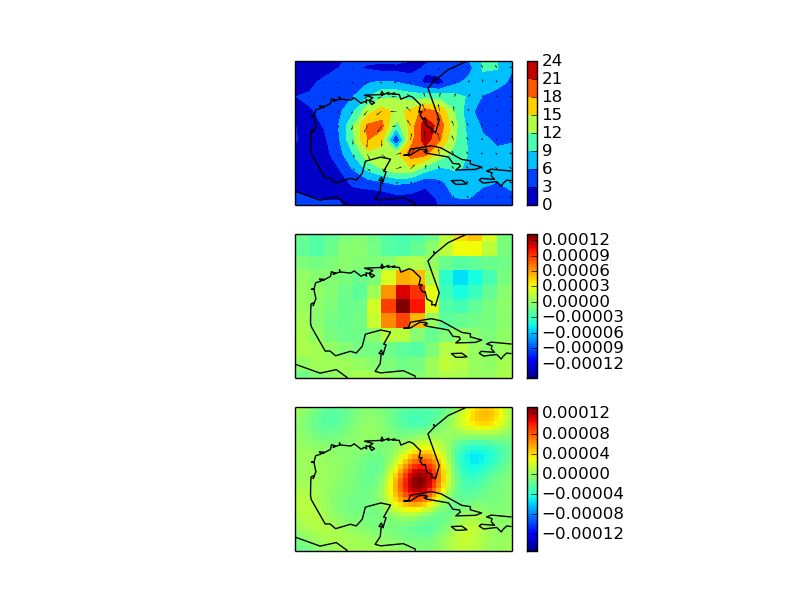
\includegraphics[width=\textwidth]{figures/katrina_data_proc}
    \caption{TODO: Caption goes here.}
    \label{fig:katrina_data_proc}
\end{figure}

\begin{figure}[hbp]
    \centering
    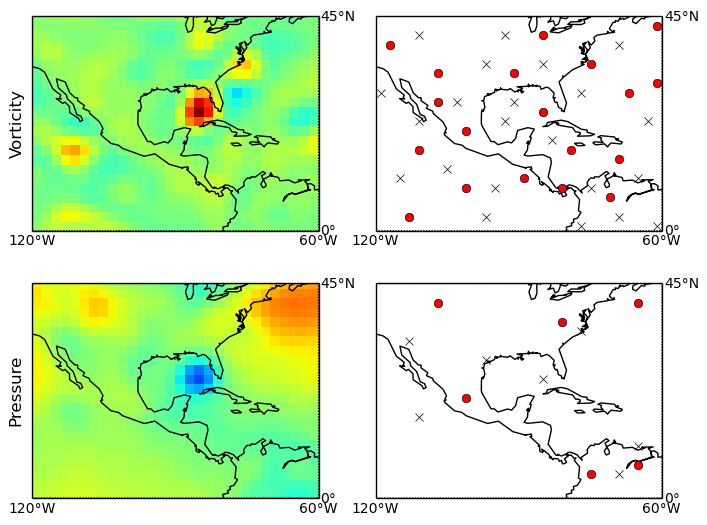
\includegraphics[width=\textwidth]{figures/katrina_max_mins}
    \caption{TODO: Caption goes here.}
    \label{fig:katrina_max_mins}
\end{figure}

\section{Tracking}

From both initial experimentation, and reading the literature \parencite{TODOmultiple}, it was found
that tracking on minima of the pressure field did not produce suitable tracks for identifying
storm systems. This was due to the pressure field being subject to synoptic scale disturbances
that mean that minima may not be present due to the surrounding gradient of this field. Whilst it is
possible to apply high pass filtering to remove these disturbances, it was decided to follow
\textcite{TODOmutliple} and produce derived tracks from the 20CRP data based on vorticity maxima.


% This section is confusing on re-reading it. I think I need to make it clearer that I'm going to
% compare different configurations.
For each timestep, the vorticity maxima were calculated, as per Section
\ref{sec:methods_maxima_minima}. This was done for both the \SI{995}{hPa} and \SI{850}{hPa} pressure
levels, and for the one, two and three times the actual 20CRP resolution, yielding a total of six
possible configurations for the tracking. These various configurations were compared, and the
results can be seen in Section \ref{sec:results_tracking}. Maxima that were below a threshold value
of \SI{2.5e-5}{s^{-1}} were not used as part of the tracking algorithm, as these represent weak maxima
that are unlikely to be part of even tropical storms. This choice is revisited in Section TODO where
some justification is given for this value.

The tracking algorithm used was a simple nearest neighbour tracking algorithm, with a modification
that counted two or more vorticity maxima that were sufficiently close as being part of the same storm
system, with the location and strength of the maximum given by the strongest of
these maxima. This cutoff distance was set as eight times the distance between the cells at
0\textdegree N, or approximately \SI{1800}{km}. This distance was found to reduce problems of
vorticity maxima merging and splitting. The algorithm worked as follows:

% TODO: flowchart?
\begin{enumerate}
    \item Detect all vorticity maxima for the first timestep. If two maxima are less than the cutoff
        distance apart, combine both maxima, taking the strength and position of the strongest of
        the two maxima
    \item Make each of the vorticity maxima in the first timestep the beginning of a derived track
        (whose length could end up being only one)
    \item Detect all vorticity maxima in the second timestep, combining close weaker maxima into
        stronger. % TODO: not totally clear that I'm talking about the combining step here.
    \item Calculate nearest neighbour in the second timestep to first timestep, and set this as the
        next member of the derived track
    \item Move onto the third timestep and repeat the process
\end{enumerate}

Whilst this algorithm is considerably less sophisticated that that of \textcite{hodges1994}, it was
found to produce sufficiently good tracks to pick up most of the best tracks in the IBTrACS dataset,
and almost all of the best tracks that were hurricanes (Section  \ref{sec:results_tracking}). A
discussion of other tracking algorithms can be found in Section \ref{sec:discussion_tracking_algs}.

\subsection{Tracking Results}
\label{sec:results_tracking}

Once tracks have been derived from the 20CRP, it is possible to match them to the corresponding best
tracks. The corresponding best track must be close the derived track in space, and its temporal
duration must overlap the duration of the derived track. In this project, an overlap of 6 timesteps,
or one and a half days, was required for there to be a match between a derived track and a best
track.  Additionally, the average distance from the derived track and the best track had to be lower
than a given threshold, taken as \SI{500}{km}. An example of a matching derived track taken from
one ensemble member and best track is shown in Figure \ref{fig:katrina_individual_match_em7}. 
% N.B. em7 is counting from 0.
This shows how the cumulative and mean distances between a derived track (from ensemble member 8)
and a best track are calculated. All matching tracks across all the ensemble members for each of the
different configurations for Hurricane Katrina are shown in Figure
\ref{fig:katrina_six_tracking_configs}. This shows a typical hurricane that makes landfall. Some
noticeable points from this figure are TODO.

\begin{figure}[hbp]
    \centering
    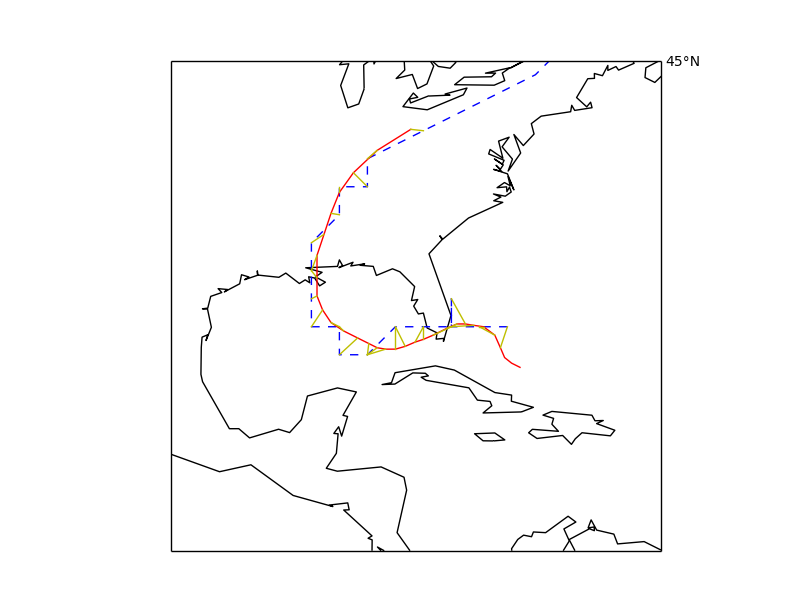
\includegraphics[width=\linewidth]{figures/katrina_individual_match_em7}
    \caption{Individual match between best track (red) and derived track (blue dashed) for Hurricane
        Katrina. The derived track was generated from the \SI{850}{hPa} pressure level using the
        original resolution and ensemble member 8. The match between the best track and the derived
        track is shown using yellow lines, which show the distance between the two tracks at each
        timestep. The cumulative distance is the sum of these distances, and the mean distance is
        the cumulative distance divided by the number of matches.
    }
    \label{fig:katrina_individual_match_em7}
\end{figure}

\begin{figure}[hbp]
    \centering
    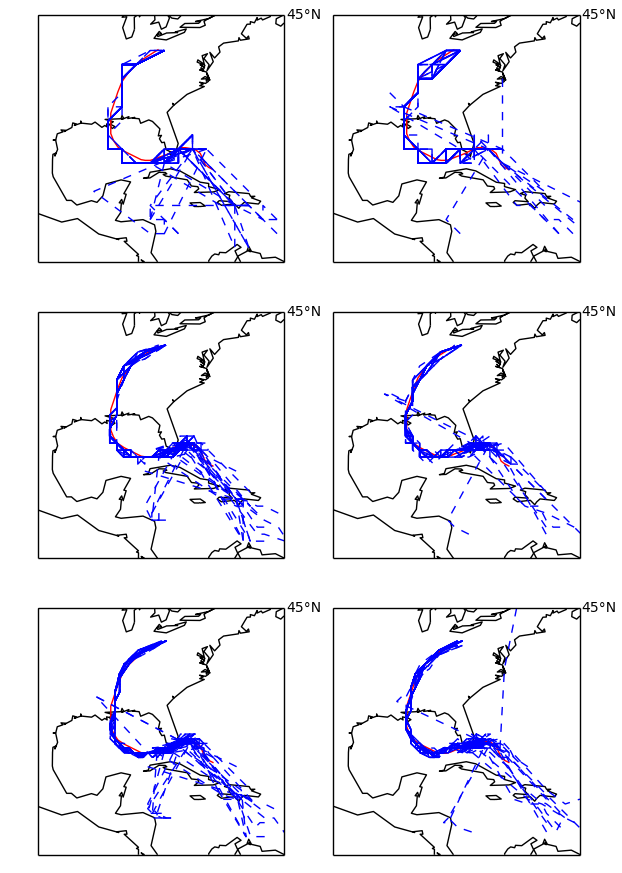
\includegraphics[width=\linewidth]{figures/katrina_six_tracking_configs}
    \caption{Caption goes here.}
    \label{fig:katrina_six_tracking_configs}
\end{figure}

To judge the tracking ability of the different tracking configurations, this matching across all
best tracks and derived tracks was done for each year in the ten year period 2000-2009.  
% TODO: switch to cumoveroverlap as it is much easier to describe.
For each year, the combined average distance between each derived track and best track was
calculated. This number was divided by the total number of matches, so as a particular configuration
that achieved relatively few matches would be penalised. This produces a metric by which the various
configurations can be judged, and each of the configurations was then compared the others to see how
they performed on this metric. The results of this comparison can be seen in Figure XX3. It is clear
that higher resolution, downscaled data produces better tracks that the unscaled data. This suggests
that for tracking, scaling of three times the original resolution should be used. What is less clear
is which is better: the \SI{995}{hPa} or the \SI{850}{hPa} pressure levels. TODO: why I picked
\SI{850}{hPa}.

% Figure XX: Comparison of wins/losses of different tracking configurations.

\newpage
\section{Extra Field Collection}

Up until this point in the processing, only the $u$ and $v$ wind fields have been utilised. From
these, the vorticity has been calculated and tracks have been derived from the maxima of these
fields.  However, to successfully classify part of a track as being of hurricane strength, it is
necessary to collect more fields. These fields will help to distinguish hurricanes from
non-hurricanes. To this end, the latitude, longitude, date and ensemble member were used to obtain
further variables from the 20CRP dataset. These variables were:

\begin{enumerate}
    \item \textbf{Minimum pressure:} the pressure minimum within \SI{1000}{km} of the vorticity
        maximum was found and the distance from the vorticity maximum to this minimum was also stored.
    \item \textbf{Ambient pressure difference:} the difference in pressure between the minimum
        pressure and the local mean pressure, as calculated by taking the surrounding 121 grid cells
        and averaging their pressures.
    \item \textbf{Temperature at \SI{995}{hPa}:} the temperature at the \SI{995}{hPa} pressure
        level.
    \item \textbf{Temperature at \SI{850}{hPa}:} the temperature at the \SI{850}{hPa} pressure
        level.
    \item \textbf{Temperature difference:} the temperature difference between the \SI{995}{hPa} and
        \SI{850}{hPa} pressure levels.
    \item \textbf{Maximum windspeed:} the maximum wind speed in the nearest 121 grid cells.
    \item \textbf{CAPE:} TODO
    \item \textbf{PWAT:} TODO
    \item \textbf{RH995:} TODO plus mention that is was found not to be that useful, and so dropped.
\end{enumerate}

Figure XX shows the pressure and vorticity fields surrounding the vorticity maxima for the Hurricane
Katrina track (taken from ensemble member YY). Figure XX shows the different fields plotted for each
timestep that Katrina was tracked for. Figure XX shows the derived pressure and maximum wind speed
for Katrina, plotted with the equivalent variables for the matching best track. From this figure, it
is clear that there is very little correlation in these two variable between the derived track and
% Check this\dots 
the best track. This is surprising, not least because the 20CRP assimilates the pressure data from
the IBTrACS dataset. Reasons as to why this might be so are examined further in XXX.

% Figure XX: one timestep per day showing wind/vorticity for Katrina.

% Figure XX: plot of all collected fields for Katrina.

% Figure XX: plot showing poor correlation between Katrina derived and best.

\section{Classification}


\chapter{20\ts{th} Century Analysis Results}
% Data analysis and results.

\chapter{Discussion}

\section{Tracking Algorithms}
\label{sec:discussion_tracking_algs}.

\chapter{Conclusions}

% Not included in word count.
\addcontentsline{toc}{chapter}{Auto-critique}
\chapter*{Auto-critique}

% Harvard style bibliography.
\addcontentsline{toc}{chapter}{References}
\printbibliography[title={References}]

%\appendix 
%\section{Additional information}

\end{document}
